%% ****** Start of file aiptemplate.tex ****** %
%%
%%   This file is part of the files in the distribution of AIP substyles for REVTeX4.
%%   Version 4.1 of 9 October 2009.
%%
%
% This is a template for producing documents for use with 
% the REVTEX 4.1 document class and the AIP substyles.
% 
% Copy this file to another name and then work on that file.
% That way, you always have this original template file to use.

%\documentclass[aip,graphicx]{revtex4-1}
%\documentclass[aip,reprint]{revtex4-1}

%\usepackage{graphicx}

%\draft % marks overfull lines with a black rule on the right
%\documentclass[pre,aps,floatfix,authordate1-4,twocolumn]{revtex4-1}
%\documentclass[pre,aps,floatfix,authordate1-4]{revtex4-1}

\documentclass[aps,prl,superscriptaddress,twocolumn]{revtex4}



%\documentclass[aps,prl,preprint,groupedaddress]{revtex4}

\usepackage{rotating} 
\usepackage{times}
\usepackage{graphicx}
\usepackage{setspace}
\usepackage{amsmath}
\usepackage{epstopdf}
\usepackage[obeyFinal]{easy-todo}
\usepackage{csquotes}
\usepackage{xr}
\externaldocument{manuscriptPSsuppl}

\begin{document}

% Use the \preprint command to place your local institutional report number 
% on the title page in preprint mode.
% Multiple \preprint commands are allowed.
%\preprint{}

\title{NMRlipids IV: Headgroup \& glycerol backbone structures, and cation binding in bilayers with PS lipids} %Title of paper

% repeat the \author .. \affiliation  etc. as needed
% \email, \thanks, \homepage, \altaffiliation all apply to the current author.
% Explanatory text should go in the []'s, 
% actual e-mail address or url should go in the {}'s for \email and \homepage.
% Please use the appropriate macro for the type of information

% \affiliation command applies to all authors since the last \affiliation command. 
% The \affiliation command should follow the other information.

\author{Pavel Buslaev}
\affiliation{Moscow Institute of Physics and Technology}
\author{Fernando Favela}
\affiliation{Mexico}
\author{Tiago M. Ferreira}
\affiliation{Halle, Germany}
\author{Ivan Gushchin}
\affiliation{Moscow Institute of Physics and Technology}
\author{Matti Javanainen}
\affiliation{Institute of Organic Chemistry and Biochemistry,
Academy of Sciences of the Czech Republic, 
Prague 6, Czech Republic}
\author{Batuhan Kav}
\affiliation{Department of Theory and Bio-Systems, Max Planck Institute of Colloids and Interfaces, 14424 Potsdam, Germany}
\author{Jesper J. Madsen}
\affiliation{Department of Chemistry, The University of Chicago, Chicago, Illinois 60637, United States of America}
\author{Markus Miettinen}
\affiliation{Department of Theory and Bio-Systems, Max Planck Institute of Colloids and Interfaces, 14424 Potsdam, Germany}
\author{Josef Melcr}
\affiliation{Institute of Organic Chemistry and Biochemistry,
Academy of Sciences of the Czech Republic, 
Prague 6, Czech Republic}
\author{Ricky Nencini}
\affiliation{Institute of Organic Chemistry and Biochemistry,
Academy of Sciences of the Czech Republic, 
Prague 6, Czech Republic}
\author{O. H. Samuli Ollila}
\email[]{samuli.ollila@helsinki.fi}
%\homepage[]{Your web page}
\affiliation{Institute of Organic Chemistry and Biochemistry,
Academy of Sciences of the Czech Republic, 
Prague 6, Czech Republic}
\affiliation{Institute of Biotechnology, University of Helsinki}
\author{Thomas Piggot   \todo{Authorlist is not yet complete}}
\affiliation{Southampton, United Kingdom}
%\author{NMRlipids collaboration}
%\affiliation{nmrlipids.blogspot.fi} 


% Collaboration name, if desired (requires use of superscriptaddress option in \documentclass). 
% \noaffiliation is required (may also be used with the \author command).
%\collaboration{}
%\noaffiliation

\date{\today}

\begin{abstract}
  % insert abstract here
Phosphatidylserine (PS) is the most common negatively
charged lipid in eukaryotic membranes.
PS lipids interact with signaling and other proteins via
electrostatic interactions and direct binding, and induce
membrane fusion and phase separation together with calcium ions.
Molecular details of these phenomena are not well understood,
because accurate models to interpret the experimental data have not
been available. Here, we collect a set of experimental NMR data that
can be used together with molecular dynamics (MD) simulations
to interpret the lipid headgroup structures and details of ion binding
in pure PS, and mixed PS:PC, lipid bilayers. We use the open collaboration
method to collect data from a wide range of available MD models of PS lipids.
None of the models reproduce the NMR data within experimental accuracy,
but the best headgroup models suggest that the carboxyl group in the serine headgroup
does not rotate freely. In line with the previous results for PC lipids,
none of the force fields correctly captures the cation binding affinity.
In contrast to PC lipids, the response of PS headgroups
to bound ions  in the tested MD simulation models
qualitatively differs from experiments. The collected experimental dataset and simulation
results pave the way for improvement of lipid force fields to correctly
describe the biologically relevant negatively charged membranes and their interactions with ions.
This work is part of the NMRlipids open collaboration project (\url{nmrlipids.blogspot.fi}).
\end{abstract}

%\pacs{}% insert suggested PACS numbers in braces on next line

\maketitle %\maketitle must follow title, authors, abstract and \pacs

% Body of paper goes here. Use proper sectioning commands. 
% References should be done using the \cite, \ref, and \label commands


%\label{}
\section{Introduction}
Phosphatidylserine (PS) is the most common negatively
charged lipid in eukaryotic membranes.
PS lipids compose 8.5\% of total lipid weight of red blood cells,
but the abundance varies between different organelles up to
25-35\% in the cytosolic leaflet of plasma membranes \cite{lemmon08,leventis10,li14}.
Despite of the relatively low abundance \todo{Relatively low compared to what?}, PS lipids
are important signaling molecules. They interact with
signaling proteins \cite{leventis10}, regulate
surface charge and protein localization \cite{yeung08}, and
induce protein aggregation \cite{zhao04,gorbenko06}.
Some protein domains interact specifically with PS lipids,
while others are attracted by nonspecific electrostatics and the
binding can be regulated by calcium \cite{leventis10}.
Therefore, the structural details
of lipid headgroups and the details of cation binding
are crucial for the PS-mediated signaling processes.

Previous experimental studies have concluded that the
PS headgroup is more rigid than the phosphatidylcholine (PC)
due to hydrogen bonding network or
electrostatic interactions \cite{browning80,buldt81}.
Multivalent cations and Li$^+$ are able to form strong
dehydrated molecular complexes with PS lipids,
while monovalent ions interact more weakly with
PS-containing bilayers \cite{hauser77,kurland79,eisenberg79,hauser83,dluhy83,hauser85,feigenson86,mattai89,roux90,roux91,boettcher11}.
The dehydrated complexes of PS headgroup and calcium ions can also lead to
phase separation \cite{hauser77,kurland79,hauser85,feigenson86,mattai89,roux90,roux91}.
On the other hand, some studies propose that the specific binding
affinity is similar for the negatively charged and zwitterionic lipids, and
the increased cation binding to negatively charged lipid bilayers arises only due
to the increased local cation concentration in the membrane vicinity~\cite{seelig90,sinn06}.
Dilution of bilayers with PC lipids makes PS headgroups
less rigid and reduces their propensity to form
strong complexes with multivalent ions~\cite{browning80,buldt81,roux90,roux91}.
The molecular level interpretation of these observations is,
however, lacking.

\begin{table*}[htb]
%\begin{sidewaystable*}[!p]
\centering
\caption{The list of MD simulations of pure PS bilayers without additional salt.
  Simulation details are given in the supplementary information
    %   The lipid force fields named as in our previous work~\cite{botan15}.
}\label{PSsystems}
%begin{minipage}[t]{\textwidth}
\begin{tabular}{l c r r r r r c c}
  %\hline
  % some footnotes are not visible in typeset-MS (pdf)
 lipid/counter-ions & force field for lipids / ions & \footnote{Number of lipid molecules with largest mole fraction}N$_{\rm l}$   &  \footnote{Number of water molecules}N$_{\rm w}$  & \footnote{Number of additional cations}N$_{\rm c}$  & \footnote{Simulation temperature}T (K)  & \footnote{Total simulation time}t$_{{\rm sim}}$(ns) & \footnote{Time used for analysis}t$_{{\rm anal}}$ (ns) &   \footnote{Reference for simulation files}files\\
    \hline
    POPS/Na$^+$  & CHARMM36 \cite{venable13} & 128 & 4480 & 0  & 298  & 500 & 100 & \cite{charmm36POPS298K} \\
    POPS/K$^+$   & CHARMM36 \cite{venable13} & 128 & 4480 & 0  & 298  & 500 & 100 & \cite{charmm36POPS298Kpotassium} \\
    POPS/Na$^+$  & CHARMM36ua \cite{??} \todoi{Correct citation for CHARMMua DOPS} & 128 & 4480 & 0  & 298  & 500 & 100 & \cite{charmm36uaPOPS298K} \\
    POPS/Na$^+$  & MacRog \cite{maciejewski14}  & 128 & 4480 & 0  & 298  & 500 & 100  & \cite{macrogPOPS298Kcorrect} \\
    POPS/K$^+$   & MacRog \cite{maciejewski14}  & 128 & 4480 & 0  & 298  & 200 & 150 & \cite{macrogPOPS298KwithK} \\
    POPS/Na$^+$  & lipid17  \cite{gould18} / JC  \cite{joung08}   & 128    & 4480   & 0   & 298  & 600 & 100 & \cite{lipid17POPSjcions} \\
    POPS/Na$^+$  & lipid17 \cite{gould18} / ff99 \cite{aqvist90}  & 128    & 4480   & 0   & 298  & 600 & 100 & \cite{lipid17POPSff99ions} \\
    POPS/Na$^+$  & Berger \cite{mukhopadhyay04,??}          & 128 & 4480 & 0  & 298  & 500 & 100 & \cite{bergerPOPS298K} \\
    POPS/Na$^+$  & GROMOS-CKPM \cite{??} \todoi{Correct citation(s) for CKP.} & 128 & 4480 & 0  & 298  & 500 & 100 & \cite{ckp1POPS303K} \\
    POPS/Na$^+$  & GROMOS-CKP \cite{??} \todoi{Correct citation(s) for CKP.}  & 128 & 4480 & 0  & 298  & 500 & 100 & \cite{ckp2POPS303K} \\
    POPS/Na$^+$  & Slipids \cite{jambeck13}  & 128 & 4480 & 0  & 298  & 500 & 100 & \cite{slipidsPOPS298K} \\
  \hline
    DOPS/Na$^+$  & CHARMM36 \cite{venable13}       & 128 & 4480 & 0  & 303  & 500 & 100 & \cite{charmm36DOPS303K} \\
    DOPS/Na$^+$  & CHARMM36ua \cite{??} \todoi{Correct citation for CHARMMua DOPS}   & 128 & 4480 & 0  & 303  & 500 & 100 & \cite{charmm36uaDOPS303K} \\
    DOPS/Na$^+$  & lipid17 \cite{gould18} / JC  \cite{joung08}    & 128    & 4480   & 0   & 303  & 600 & 100 & \cite{lipid17DOPSjcions} \\
    DOPS/Na$^+$  & lipid17 \cite{gould18} / ff99 \cite{aqvist90}  & 128    & 4480   & 0   & 303  & 600 & 100 & \cite{lipid17DOPSff99ions} \\
    DOPS/Na$^+$  & Berger \cite{mukhopadhyay04,??}    & 128  & 4480  & 0  & 303  & 500 & 100 & \cite{bergerDOPS303K} \\
    DOPS/Na$^+$  & GROMOS-CKPM \cite{??} \todoi{Correct citation(s) for CKP.} & 128 & 4480 & 0  & 303  & 500 & 100 & \cite{ckp1DOPS303K} \\
    DOPS/Na$^+$  & GROMOS-CKP  \cite{??} \todoi{Correct citation(s) for CKP.} & 128 & 4480 & 0  & 303  & 500 & 100 & \cite{ckp2DOPS303K} \\
    DOPS/Na$^+$  & Slipids \cite{jambeck13}        & 128 	& 4480  & 0  & 303  & 500 & 100 & \cite{slipidsDOPS303K} \\
    DOPS/Na$^+$  & Slipids \cite{jambeck13}        & 288 	& 11232 & 0  & 303  & 200 & 100 & \cite{slipidsDOPSfiles} \\
    \end{tabular}
%\end{minipage}
%\end{sidewaystable*} 
\end{table*}

Several classical molecular dynamics (MD) simulation studies have been done
to understand the PS headgroups, their influence on lipid bilayer properties, and their
interaction with
ions \cite{cascales96,pandit02,mukhopadhyay04,pedersen06,vernier09,boettcher11,molina12,jurkiewicz12,venable13,pan14,vangaveti14,melcrova16,valentine18,hallock18}.
However, the results have depended strongly on the force field used.
For example, recent simulations using the NBfix parameters for calcium \cite{kim16} in
CHARMM36 force field \cite{klauda10,venable13}, combined with 2D infrared spectroscopy,
suggest that calcium ions interact only with the carboxylate group of PS lipids \cite{valentine18}; in contrast,
the same force field without the NBfix parameters, combined with NMR chemical shifts and
REDOR \todo{Spell out REDOR?} experiments, suggests a significant binding affinity also to the phosphate region \cite{hallock18}.
On the other hand, simulations with the Berger force field \cite{berger97,mukhopadhyay04},
combined with fluorescent and vibrational sum frequency spectroscopy, suggest a significant
calcium binding also to the carbonyls in the acyl chains \cite{melcrova16}.
We have recently demonstrated that such controversies can be resolved by
comparing the C--H bond order parameters, $S_\mathrm{CH}$, of lipid headgroups between simulations
and experiments \cite{botan15,catte16}. The $S_\mathrm{CH}$ can be directly
measured from NMR experiments with high accuracy and compared to simulations
in order to evaluate the simulation model quality or to interpret the experiments \cite{ollila16}.
Previous studies showed that the structure of PC lipid headgroup and glycerol backbone are not well
captured by most MD force fields~\cite{botan15}, and that the cation binding to PC
lipid bilayers is overestimated \cite{catte16}.
%
Based on these data, the cation binding affinity to POPC bilayer has since been improved by implicitly including the electronic polarizability using the electronic continuum correction \cite{melcr18}.
\todo{Should we leave the mention of ECC out from the Introduction
(i.e., mention it only in the Conclusions) as the ECC parameters are not used in the paper?} 

Here, we collect a set of experimentally measured lipid headgroup and
glycerol backbone C--H bond order parameters, which can be used to
evaluate the quality of headgroup structure and ion binding affinity
in MD simulations of lipid bilayers containing PS lipids. 
The available MD simulation models of PS are then compared with
the collected experimental data.
%using the NMRlipids open collaboration project (\url{nmrlipids.blogspot.fi}).
The results pave the way
for development of lipid force fields with realistic description of
the headgroup region of negatively charged lipids in physiological salt
conditions. Such models are expected to be useful in understanding
biological function of lipid headgroups and glycerol backbone, as
these behave similarly in model membranes and in bacterial cells \cite{gally81,scherer87,seelig90}.



\begin{table*}[tb]
%\begin{sidewaystable*}[!p]
\centering
\caption{The list of POPC:POPS mixtures simulated with different molar fractions and different amounts of added calcium. 
  The salt concentrations are calculated as [salt]=N$_{\rm c} \times$[water]\,/\,N$_{\rm w}$, where [water]\,=\,55.5~M.
  This corresponds the concentration in buffer before solvating lipids, which are
  reported in the experiments by Roux et al.~\cite{roux90}.
  The simulation details are given in the supplementary information.
   % The lipid force fields named as in our previous work~\cite{botan15}.
}\label{mixedIONsystems}
%begin{minipage}[t]{\textwidth}
\begin{tabular}{l c c c c c c c c c }
  lipid/counter-ions & force field for lipids / ions & [CaCl$_2$]\,(M)  &  \footnote{Number of lipid molecules with largest mole fraction}N$_{\rm l}$   &  \footnote{Number of water molecules}N$_{\rm w}$   & \footnote{Number of additional cations}N$_{\rm c}$  & \footnote{Simulation temperature}T (K)  & \footnote{Total simulation time}t$_{{\rm sim}}$(ns) & \footnote{Time used for analysis}t$_{{\rm anal}}$ (ns) &   \footnote{Reference for simulation files}files\\
  \hline
%    POPC:POPS (5:1)/K$^+$  & CHARMM36 \cite{klauda10,venable13} &0  & 110:22 & 4935 & 0  & 298  & 100 & 100 \todoi{Equilibration?} & \cite{charmm36pops+83popcT298K}  \\
    POPC:POPS (5:1)/K$^+$  & CHARMM36 \cite{klauda10,venable13} &0 & 250:50 & 11207 & 0  & 298  & 200 & 180   & \cite{POPC5POPS1noCaClCHARMM}  \\
    POPC:POPS (5:1)/K$^+$  & CHARMM36 \cite{klauda10,venable13} &0 & 110:22 & 4620  & 0  & 298  & 500 & 100 & \cite{charmm36pops+83popcT298Kpiggot}  \\
    POPC:POPS (5:1)/Na$^+$ & CHARMM36 \cite{klauda10,venable13} &0 & 110:22 & 4620  & 0  & 298  & 500 & 100 & \cite{charmm36pops+83popcT298KpiggotSODIUM}  \\
    POPC:POPS (5:1)        & CHARMM36 \cite{klauda10,venable13,kim16}  & 0.26 & 250:50  & 11190  & 53  & 298  & 200 & 180 & \cite{POPC5POPS1withCaClCHARMM}   \\
    POPC:POPS (5:1)        & CHARMM36 \cite{klauda10,venable13,kim16}  & 1.06 & 250:50  & 11174  & 214  & 298  & 200 & 180  & \cite{POPC5POPS1with1MCaClCHARMM}  \\
    POPC:POPS (1:1)/K$^+$  & CHARMM36 \cite{klauda10,venable13}        & 0    & 150:150 & 10785    & 0  & 298  & 200 & 180   & \cite{POPC1POPS1noCaClCHARMM}  \\
  \hline
    POPC:POPS (1:0)        & MacRog \cite{maciejewski14} &0    & 120:0  & 5120 & 0    & 298  & 200 & 150 & \cite{macrogPOPC298K}  \\
    POPC:POPS (5:1)/K$^+$  & MacRog \cite{maciejewski14} &0    & 120:24 & 5760 & 0    & 298  & 400 & 250 & \cite{POPCpopsMACROG}  \\
    POPC:POPS (5:1)/K$^+$  & MacRog \cite{maciejewski14} & 0.10 & 120:24 & 5760 & 10   & 298  & 600 & 300 & \cite{POPCpopsMACROG}  \\
    POPC:POPS (5:1)/K$^+$  & MacRog \cite{maciejewski14} & 0.30 & 120:24 & 5760 & 31   & 298  & 600 & 300  & \cite{POPCpopsMACROG}  \\
    POPC:POPS (5:1)/K$^+$  & MacRog \cite{maciejewski14} & 1.00   & 120:24 & 5760 & 104  & 298  & 600 & 300  & \cite{POPCpopsMACROG}  \\
    POPC:POPS (5:1)/K$^+$  & MacRog \cite{maciejewski14} & 3.00   & 120:24 & 5760 & 311  & 298  & 600 & 300  & \cite{POPCpopsMACROG}  \\
%    POPC:OPPS (5:1)/K$^+$  & MacRog \cite{maciejewski14} &4.00    & 0   & 120:24 & 5760 & 415  & 298  & 300 & 200 & \cite{POPCpopsMACROGwithK}  \\
    \hline
    POPC:POPS (5:1)/K$^+$  & Lipid14/17 \cite{dickson14,gould18}  & 0      & 120:24 & 5760 & 0   & 298  & 500 & 200 & \cite{POPCpopsLIPID17withKCI}  \\
    POPC:POPS (5:1)/Na$^+$  & Lipid14/17 \cite{dickson14,gould18} & 0      & 120:24 & 5760 & 0   & 298  & 500 & 200 & \cite{POPCpopsLIPID17withNaCI}  \\
    POPC:POPS (5:1)         & Lipid14/17 \cite{dickson14,gould18} &0.50    & 120:24 & 5760 & 52   & 298  & 300 & 200 & \cite{POPCpopsLIPID17withCaCl}  \\
    POPC:POPS (5:1)  & Lipid14/17 \cite{dickson14,gould18}        &1.00    & 120:24 & 5760 & 104   & 298  & 300 & 200 & \cite{POPCpopsLIPID17withCaCl}  \\
    POPC:POPS (5:1)  & Lipid14/17 \cite{dickson14,gould18}        &2.00    & 120:24 & 5760 & 208   & 298  & 300 & 200 & \cite{POPCpopsLIPID17withCaCl}  \\
    POPC:POPS (5:1)  & Lipid14/17 \cite{dickson14,gould18}        &3.00    & 120:24 & 5760 & 311   & 298  & 300 & 200 & \cite{POPCpopsLIPID17withCaCl}  \\
    POPC:POPS (5:1)  & Lipid14/17 \cite{dickson14,gould18}        &4.00    & 120:24 & 5760 & 415   & 298  & 300 & 200 & \cite{POPCpopsLIPID17withCaCl}  \\
    POPC:POPS (5:1)/Na$^+$ & Lipid14/17 \cite{dickson14,gould18}  & 0      & 60:12 & 3600  & 0   & 298  & 1000  & 1000  & \cite{lipid17_cacl_series}   \\
    POPC:POPS (5:1)/Na$^+$ & Lipid14/17 \cite{dickson14,gould18,smith94,dang06}  & 0.08   & 60:12 & 3561  & 5   & 298  & 1000  & 1000  & \cite{lipid17_cacl_series}   \\
    POPC:POPS (5:1)/Na$^+$ & Lipid14/17 \cite{dickson14,gould18,smith94,dang06}  & 0.13   & 60:12 & 3561  & 8   & 298  & 1000  & 1000  & \cite{lipid17_cacl_series}   \\
    POPC:POPS (5:1)/Na$^+$ & Lipid14/17 \cite{dickson14,gould18,smith94,dang06}  & 0.20   & 60:12 & 3561  & 13  & 298  & 1000  & 1000  & \cite{lipid17_cacl_series}   \\
    POPC:POPS (5:1)/Na$^+$ & Lipid14/17 \cite{dickson14,gould18,smith94,dang06}  & 0.41   & 60:12 & 3522  & 26  & 298  & 1000  & 1000  & \cite{lipid17_cacl_series}   \\
    POPC:POPS (5:1)/Na$^+$ & Lipid14/17 \cite{dickson14,gould18,smith94,dang06}  & 0.62   & 60:12 & 3483  & 39  & 298  & 1000  & 1000  & \cite{lipid17_cacl_series}   \\
    \hline
    POPC:POPS (4:1)/Na$^+$  & Berger \cite{tieleman99,mukhopadhyay04}  & 0   & 102:26 & 4290 & 0   & 310  & 120 & 80 & \cite{bergerPOPSPOPC4:1mixtureT310K}  \\
    POPC:POPS (4:1)  & Berger \cite{tieleman99,mukhopadhyay04}         & 0.102\footnote{Calculation of concetration complicated due the scaled ions. Concentration taken as reported in the delivered data.}   & 104:24 & 4306 & 24 & 310  & 300 & 100 & \cite{POPCpopsBERGERwith102mMCa}  \\
    POPC:POPS (4:1)  & Berger \cite{tieleman99,mukhopadhyay04}         & 0.715\footnote{Calculation of concetration complicated due the scaled ions. Concentration taken as reported in the delivered data.}  & 104:24 & 4306 & 72 & 310  & 300 & 100 & \cite{POPCpopsBERGERwith715mMCa}  \\
    \hline
    POPC:POPS (5:1)/Na$^+$  & GROMOS-CKP \cite{??}             & 0     & 110:22 & ?     & 0  & 298  & 500 & 100 & \cite{POPCpopsGROMOSCKPwithNa}  \\
    POPC:POPS (5:1)/Na$^+$  & GROMOS-CKPM \cite{??}            & 0     & 110:22 & ?     & 0  & 298  & 500 & 100 & \cite{POPCpopsGROMOSCKPMwithNa}  \\
\end{tabular}
%\end{minipage}
%end{sidewaystable*} 

\end{table*}



\section{Methods}

\subsection{C--H bond order parameters from the natural abundance $^{13}$C\,NMR}

Headgroup and glycerol backbone C--H bond order parameters of POPS
were determined from the chemical-shift resolved dipolar splittings
measured with a R-type Proton Detected Local Field (R-PDLF) experiment~\cite{dvinskikh04}.
The corresponding order parameter signs were measured with a S-DROSS experiment~\cite{gross97}
using natural abundance $^{13}$C solid state NMR spectroscopy as described previously \cite{ferreira13,ferreira16}.
The experiments were done in a Bruker Avance III 400 spectrometer operating at a $^1$H Larmor frequency of 400.03 MHz.
Magic angle spinning (MAS) of the sample was used at a frequency of 5.15 kHz (R-PDLF experiment) and 5 kHz (S-DROSS experiment).
The following experimental setups were used.

{\emph{C--H bond order parameters from the R-PDLF experiment.}} The parameters are described according to Figures 1c and 2c of the original reference
for the R-PDLF experiment~\cite{dvinskikh04}.  The refocused-INEPT delays were $\tau_1=$\,1.94\,ms and $\tau_2=$\,0.97\,ms.
Radio frequency pulses with the nutation frequencies: 46.35 kHz (R18$^7_1$ pulses), 63.45 kHz ($^{13}$C 90$^{\rm{o}}$ and 180$^{\rm{o}}$),
50 kHz (SPINAL64 $^1$H decoupling pulses).
\todo{Verb missing. Would it be correct to say: 'Radio frequency pulses had the nutation frequencies:'?}
The $t_1$ increment was equal to 10.79 $\mu$s $\times18\times2$, and 32 points in the indirect
dimension were recorded using 1024 scans for each, with a recycle delay of 5\,s and a spectral with \todo{'with' $\to$ 'width'?} of 149.5 ppm.

\emph{Order parameter signs from the S-DROSS experiment.}
The parameters are described according to Figures 1b and 1c of the original reference for the S-DROSS
experiment~\cite{gross97}. The refocused-INEPT delay $\delta_2$ was 1.19 ms. The $\tau_1$ and $\tau_2$ in the S-DROSS recoupling
blocks $R$ were set as $\tau_1=$\,39.4\,$\mu$s and $\tau_2=$\,89.4 $\mu$s. Radio frequency pulses with the nutation
frequencies: 63.45 kHz ($^{13}$C 90$^{\rm{o}}$ and 180$^{\rm{o}}$), 50 kHz ($^1$H\,SPINAL64 decoupling).
\todo{Verb missing. Would it be correct to say: 'Radio frequency pulses had the nutation frequencies:'?}
The $t_1$ increment (dipolar recoupling dimension) was 800 $\mu$s, and a total of 8 points along $t_1$ were
measured using 1024 scans for each, with a recycle delay of 5\,s and a spectral with \todo{'with' $\to$ 'width'?}  of 149.5 ppm.

\emph{Numerical simulations of S-DROSS curves.}
The numerical simulations of S-DROSS curves were performed with the SIMPSON simulation package \cite{bak00}
using as input the $^{13}$C--$^1$H
dipolar couplings, either as determined by the R-PDLF experiments, or as calculated from the known $^2$H quadrupolar couplings \cite{browning80}.
The chemical shift anisotropy and homonuclear couplings were neglected, and the input file {\it{rep2000}} was used to simulate a random
distribution of bilayer orientations in the samples studied.

\emph{Sample preparation.}
The sample was prepared simply by mixing the POPS \todo{From some company?} with water (lipid:water 60:40\,wt-\%) in an Eppendorf
tube by mixing and centrifuging the sample repeatedly until a \todo{visually(?)} homogeneous viscous fluid was obtained.
Then 20 mg of the sample was  transferred to an NMR insert suitable for 4 mm NMR rotors.  
\todo{Maybe we need little bit more information about the mixing procedure?} 


\subsection{Molecular dynamics simulations}
Molecular dynamics simulation data were collected using
the Open Collaboration method \cite{botan15}, with
the NMR\-lipids Project blog (\url{nmrlipids.blogspot.fi}) and
GitHub repository (\url{github.com/NMRlipids/NMRlipidsIVotherHGs})
as the communication platforms.
The simulated systems are listed in 
Tables \ref{PSsystems} (pure PS bilayers without additional ions) 
and \ref{mixedIONsystems} (mixed PC:PS bilayers at various salt concentrations).
Further simulation details are given in the SI.
The simulation data are also indexed in a
searchable database available at \url{www.nmrlipids.fi},
and in the NMRlipids/MATCH repository (\url{github.com/NMRlipids/MATCH}).

The C--H bond order parameters were calculated directly
from the carbon and hydrogen positions using the definition
\begin{equation}
S_{\rm CH}=\frac{1}{2}\langle 3\cos^2\theta -1 \rangle,
\end{equation}
where $\theta$ is the angle between the C--H bond and the membrane normal
(taken to align with $z$, with bilayer periodic in the $xy$-plane).
Angular brackets denote average over all sampled configurations.
The order parameters were first calculated averaging over time separately
for each lipid in the system. The average and
the standard error of the mean were then calculated over different lipids.
Python program ({\tt scripts/calcOrderParameters.py}) that uses the
MDAnalysis library \cite{agrawal11,gowers16} is available in Ref. \citenum{MATCHgit}. 
The number density profiles were calculated using the {\tt gmx density} tool
of the Gromacs sofware package \cite{gromacsMANUAL}.

\subsection{Comparison of ion binding to negatively charged lipid bilayers 
between simulations and experiments using the molecular electrometer}

As the order parameters of the $\alpha$ and $\beta$ carbons in the PC headgroup
decrease proportionally to the amount of positive
charge bound to the bilayer \cite{akutsu81,altenbach84,seelig87},
they can be used to measure the ion binding affinity.
This concept, known as the molecular electrometer, is especially useful for 
comparison between simulations and experiments, as
the headgroup order parameters at varying cation
concentrations can be directly calculated from 
simulations and compared to the corresponding experimental data~\cite{catte16}. The headgroup order parameters
of negatively charged PS and PG lipids also exhibit systematic, but less
understood dependencies on the bound charge~\cite{borle85,macdonald87,roux86,roux90}.
Therefore, the ion binding affinity to negatively charged bilayers
can be better characterized by measuring the PC headgroup order parameters from 
mixed bilayers~\cite{roux86,roux90,roux91}, see section \ref{electrometerFORmixtures} in the supplementary information.

Before using the PC headgroup order parameters to quantify the ion binding
affinity, it is important to quantify their response to a known amount of bound charge~\cite{catte16,melcr18}.
This can be done using experimental data from mixtures of
monovalent cationic surfactants (dihexadecyldimethylammonium) and POPC~\cite{scherer89,melcr18},
see section \ref{electrometerCALIBRATION} in the supplementary information.
In this work, we also quantify the response of PC headgroup order parameters
to the negatively charged PS headgroups, which also follows the molecular electrometer
concept in experiments~\cite{scherer87},
see section \ref{electrometerFORmixtures} in the supplementary information.

In the experimental $^2$H~NMR literature data used in this work~\cite{browning80,roux90},
the lipids were first solvated to the buffer and then centrifuged to a pellet that
was used in the measurements. Such samples have a lower lipid concentration
(approximately 10~wt~\% of lipids~\cite{browning80,roux88,roux90}) than 
gravimetric samples (60~wt~\%) and simulations (approximately 50-60~wt~\%) in this work.
Larger multilamellar repeat distances are expected in the samples with lower lipid
concentrations due to the swelling caused by electrostatic repulsion in pure PS lipid systems~\cite{millman82}.
However, the PS headgroup order parameters measured from gravimetric samples in this work
are in good agreement with the results from centrifuged samples in the literature~\cite{browning80} (Fig.~\ref{HGorderParameters}).
Furthermore, the equilibrium repeat distance rapidly decreases with the addition of monovalent
salts, and is close to the typical simulation box sizes already above 500~mM concentrations~\cite{millman82,rand89}.
Therefore, the hydration levels of multilamellae are expected to be sufficiently similar
in the used simulations and reference experiments.

Two different definitions for the salt concentrations have been used when the molecular
electrometer concept is applied to study ion binding affinities.
The concentrations are reported either in water before solvating the lipids \cite{akutsu81,roux90,catte16},
or in bulk water after solvating the lipids \cite{altenbach84,melcr18}.
In this work, we use the former definition to be consistent with the reference
experimental data \cite{roux90}. The choice of definition has only a marginal effect
to the results in simulations with realistic ion binding affinity
(section \ref{concentrationDEFsection} in the supplementary information).

\section{Results and Discussion}

\subsection{Headgroup and glycerol backbone order parameters of POPS from $^{13}$C NMR}

\begin{figure}[!tb]
  \centering
  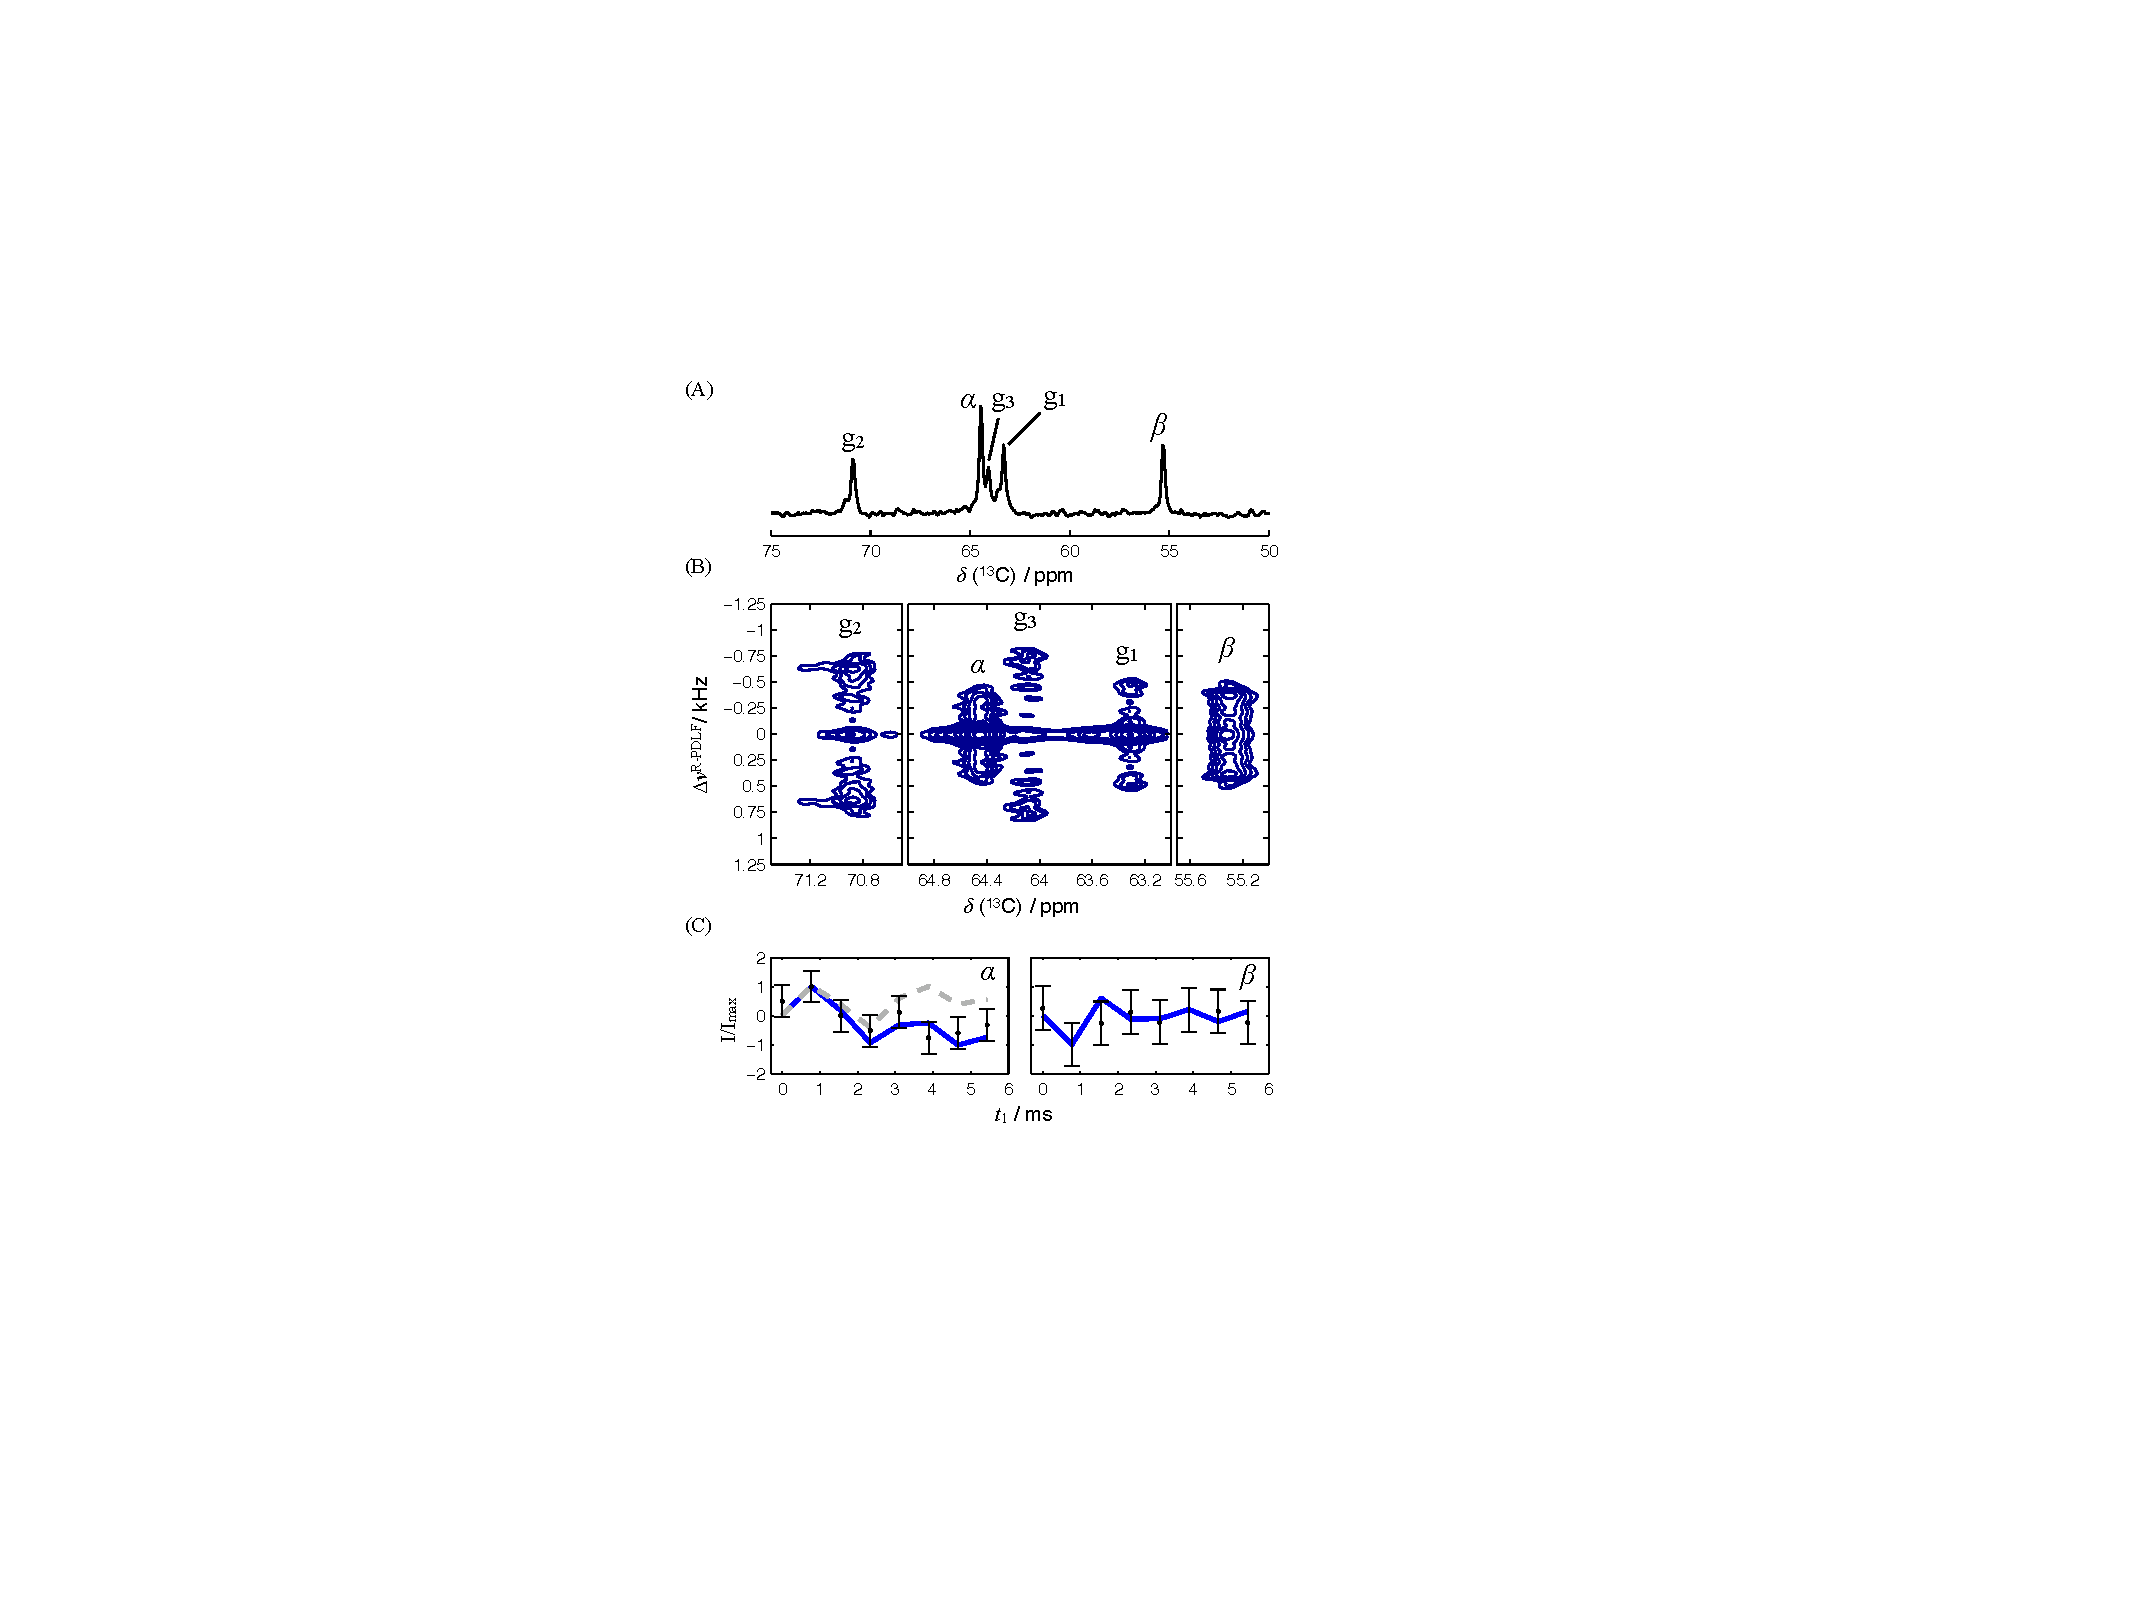
\includegraphics[width=8.5cm]{../Figs/fig1_POPS.pdf}
  \caption{\label{PShgSIGNSsimpson}
    The headgroup and glycerol backbone region of the (A) INEPT spectrum and
    (B) 2D R-PDLF spectra.
    (C) Experimental S-DROSS data (points), and SIMPSON simulations (blue lines) with
    the order parameter values of -0.12 for the $\beta$-carbon, and 0.09 and -0.02
    for the $\alpha$-carbon splittings.
    Dashed gray line is the S-DROSS curve from a SIMPSON simulation with a positive value (+0.02) 
    for the smaller $\alpha$-carbon order parameter.
  }
  \todo{I think that the peak labeling would be good to show also in (A).}\\
  \todo{Also for $\alpha$ these are OPs, right,  thus we could just exclude the word 'splittings'?}
  \todo{Please confirm: Was the positive value used for $\alpha$ in the gray curve 0.02?}
\end{figure}
\begin{figure}[!htb]
  \centering
  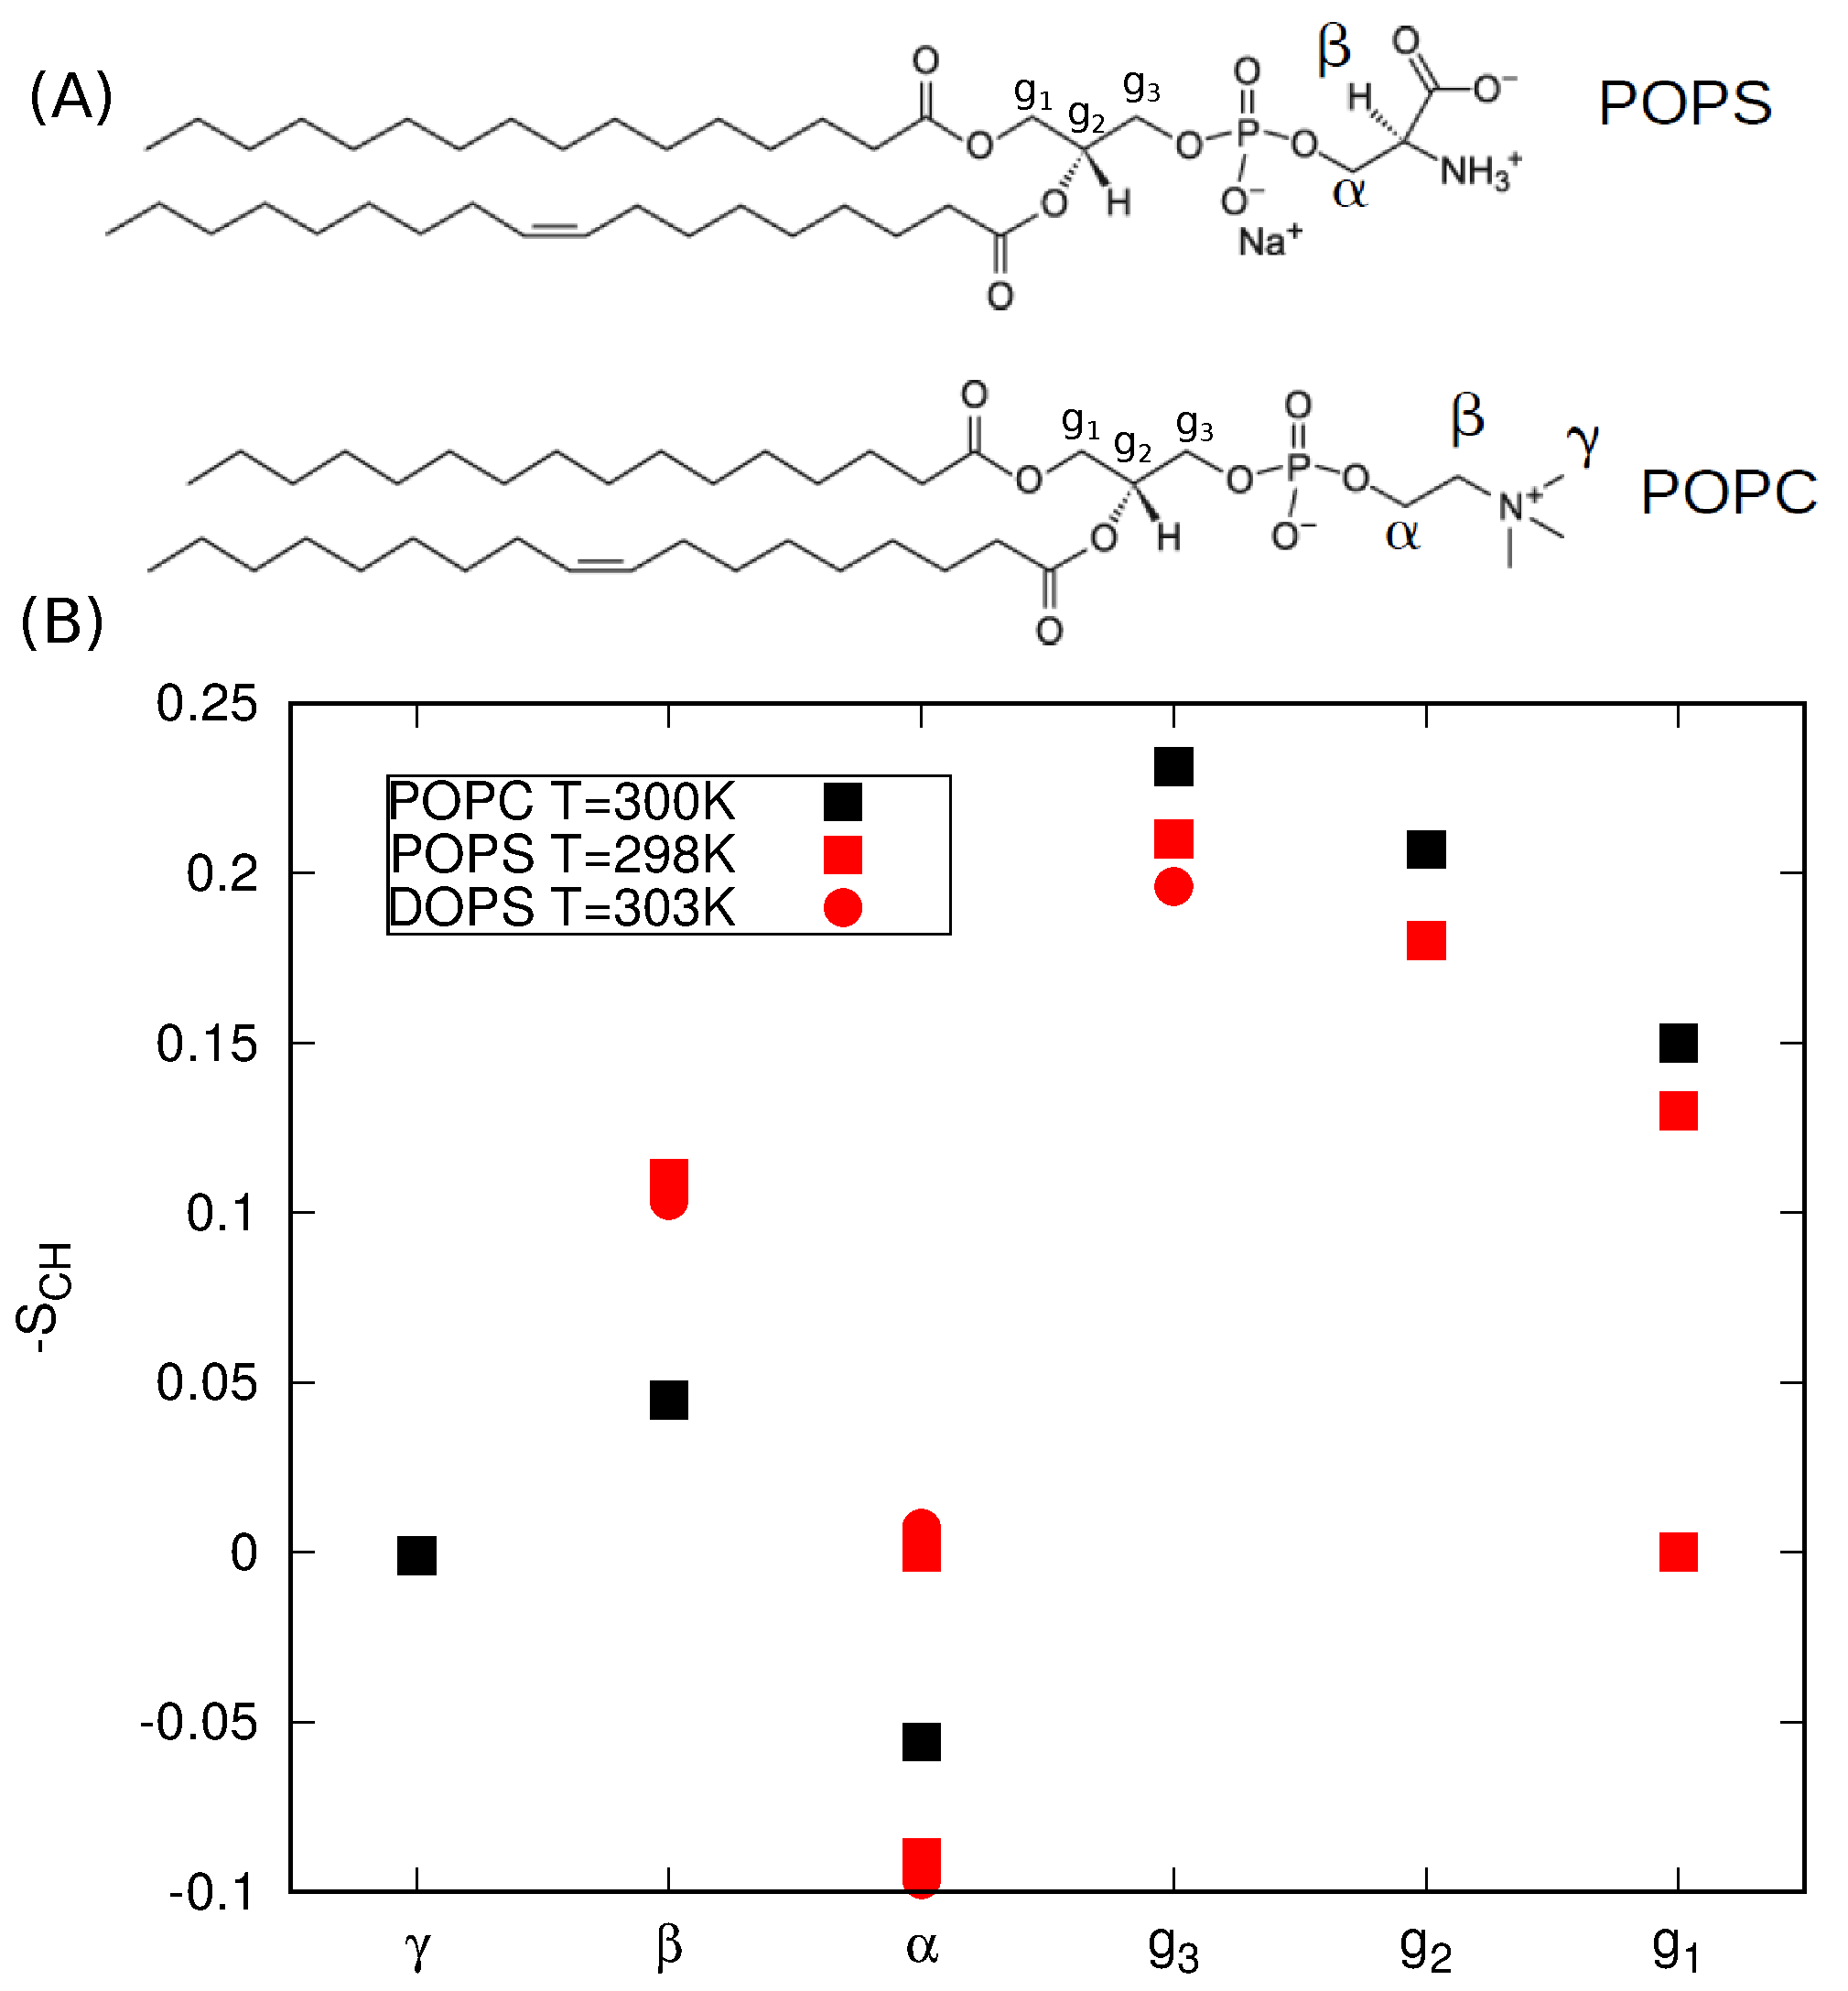
\includegraphics[width=9.0cm]{../Figs/PCPScomp.eps}
  \caption{\label{HGorderParameters}
    (A) Chemical structures and labels for the headgroup and glycerol backbone carbons.
    (B) Headgroup and glycerol backbone order parameters of POPS (T = 298 K) measured in this work compared
    with the previously published values from DOPS (T = 303 K, $^2$H NMR, 0.1M of NaCl) \cite{browning80} and 
    POPC  (T = 300 K, $^{13}$C NMR) \cite{ferreira13} experiments. Signs of the PS order parameters
    are measured in this work. Signs of the PC order parameters are measured previously~\cite{ferreira16}.
  }\todo{
  1) Use diamonds for DOPS, spheres for POPS.
  2) Error bars?
  3) Change the y-label to $S_\mathrm{CH}$, and invert the y-axis, as in Fig. 3.
  4) Make lower g1 POPC visible, e.g., by slightly larger point.
  }
\end{figure}

The INEPT and 2D R-PDLF experiments from POPS sample give well resolved spectra for all the
carbons in the headgroup and glycerol backbone regions (Fig. \ref{PShgSIGNSsimpson}).
The glycerol backbone carbon peaks were assigned according to the POPC spectra~\cite{ferreira13}.
The peaks for $\beta$ and $\alpha$ carbons were assigned according to the
known order parameters from the $^2$H\,NMR experiments~\cite{browning80}.
Slices of the R-PDLF spectra and the resulting order parameter values
are shown in the supplementary information (Fig. \ref{DPslices}). 
Since the R-PDLF and previous $^2$H\,NMR experiments \cite{browning80,roux91} give 
only the absolute values of order parameters, we determined the signs of the PS headgroup
order parameters using the S-DROSS experiment \cite{gross97}.
The S-DROSS slice clearly shows that the order parameter of
the $\beta$-carbon is negative (Fig. \ref{PShgSIGNSsimpson} C)), \todo{
Could we explain in a few words how this is clearly seen?}
which is confirmed by SIMPSON simulations. The beginning of the S-DROSS slice
suggests that the larger order parameter of the $\alpha$-carbon 
is positive and the deviation towards negative values with longer T$_1$ times suggests
that the smaller order parameter is negative. This is confirmed by a SIMPSON simulation
using the value of -0.02 from $^2$H\,NMR experiment \cite{roux91} for the smaller order parameter.
The literature value was used because the
resolution of our experiment was not sufficient to determine the
small value of the order parameter.
The S-DROSS curve from SIMPSON simulation with a positive value for the smaller order parameter
(dashed grey in Fig. \ref{PShgSIGNSsimpson} C)) did not agree with the experiment, 
confirming \todo{Or rather 'corroborating'?}
the interpretation that the smaller order parameter is negative.

\begin{figure}[]
  \centering
  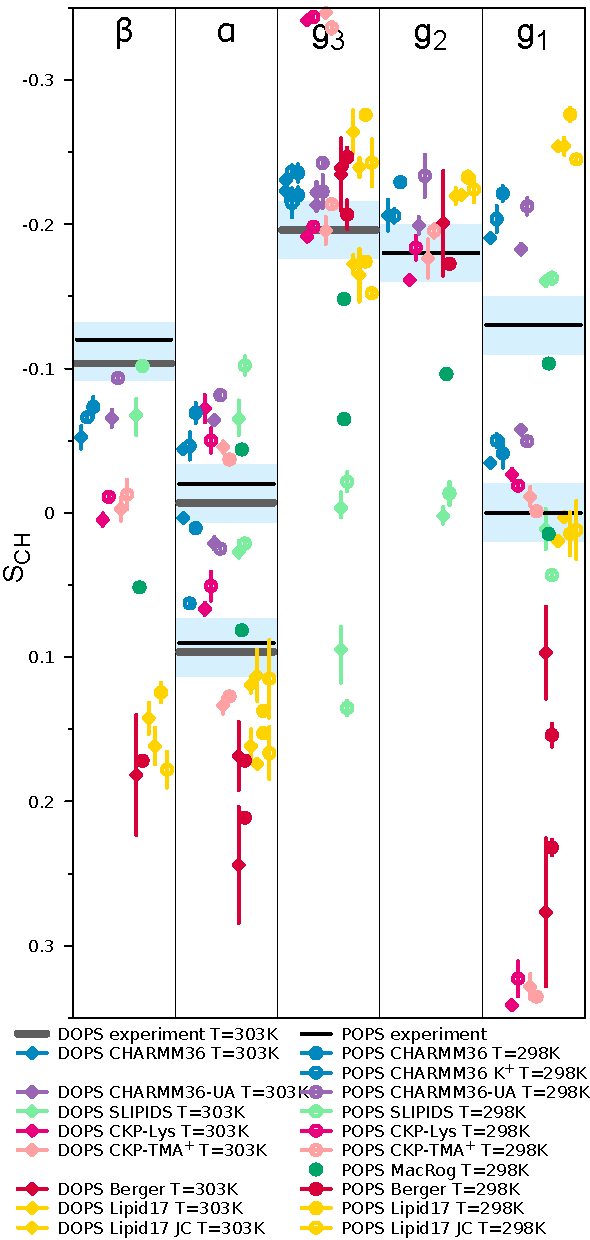
\includegraphics[width=9.0cm]{../Figs/HGorderparametersPS.pdf}
  \caption{\label{HGorderParametersPS}
    Order parameters of PS headgroup ($\beta$ and $\alpha$) and
    glycerol backbone (g$_3$, g$_2$, g$_1$) from NMR experiments (horizontal lines),
    and MD simulations with different force fields (dots).
    Experimental data for DOPS are measured with 0.1~M of NaCl~\cite{browning80},
    while all the other data are without additional salt.
    All the data for DOPS at 303~K and all the data for POPS at 298~K.
    Light blue areas span 0.04 units around the average of the extremal experimental values,
    in accordance with the expected quantitative accuracy of experimental values~\cite{ollila16}.
    The vertical bars shown for all simulation values except MacRog~K$^+$
    are not error bars, but demonstrate that for these systems
    we had at least two data sets; the ends of the bars mark the extreme values
    from the sets, and the dot marks their measurement-time-weighted average.
  }
\end{figure}


The headgroup and glycerol backbone order parameters of 
POPS measured in this work are in good agreement with the previously reported
values from $^2$H\,NMR experiments of DOPS \cite{browning80} (Fig. \ref{HGorderParameters}).
When compared with the previously measured values for POPC \cite{ferreira13} (Fig. \ref{HGorderParameters}),
the $\beta$-carbon order parameter is significantly more negative and $\alpha$-carbon
experiences a significant forking (different order parameters for the two hydrogens in the same carbon \cite{ollila16}) in the PS headgroup.
These features have been intepreted to arise from a rigid PS headgroup
conformation, stabilized by hydrogen bonds or electrostatic
interactions \cite{browning80,buldt81}, but detailed structrural interpretation is not
available. 




\subsection{Headgroup and glycerol backbone in simulations of PS lipid bilayers without additional ions}

\begin{figure}[]
  \centering
  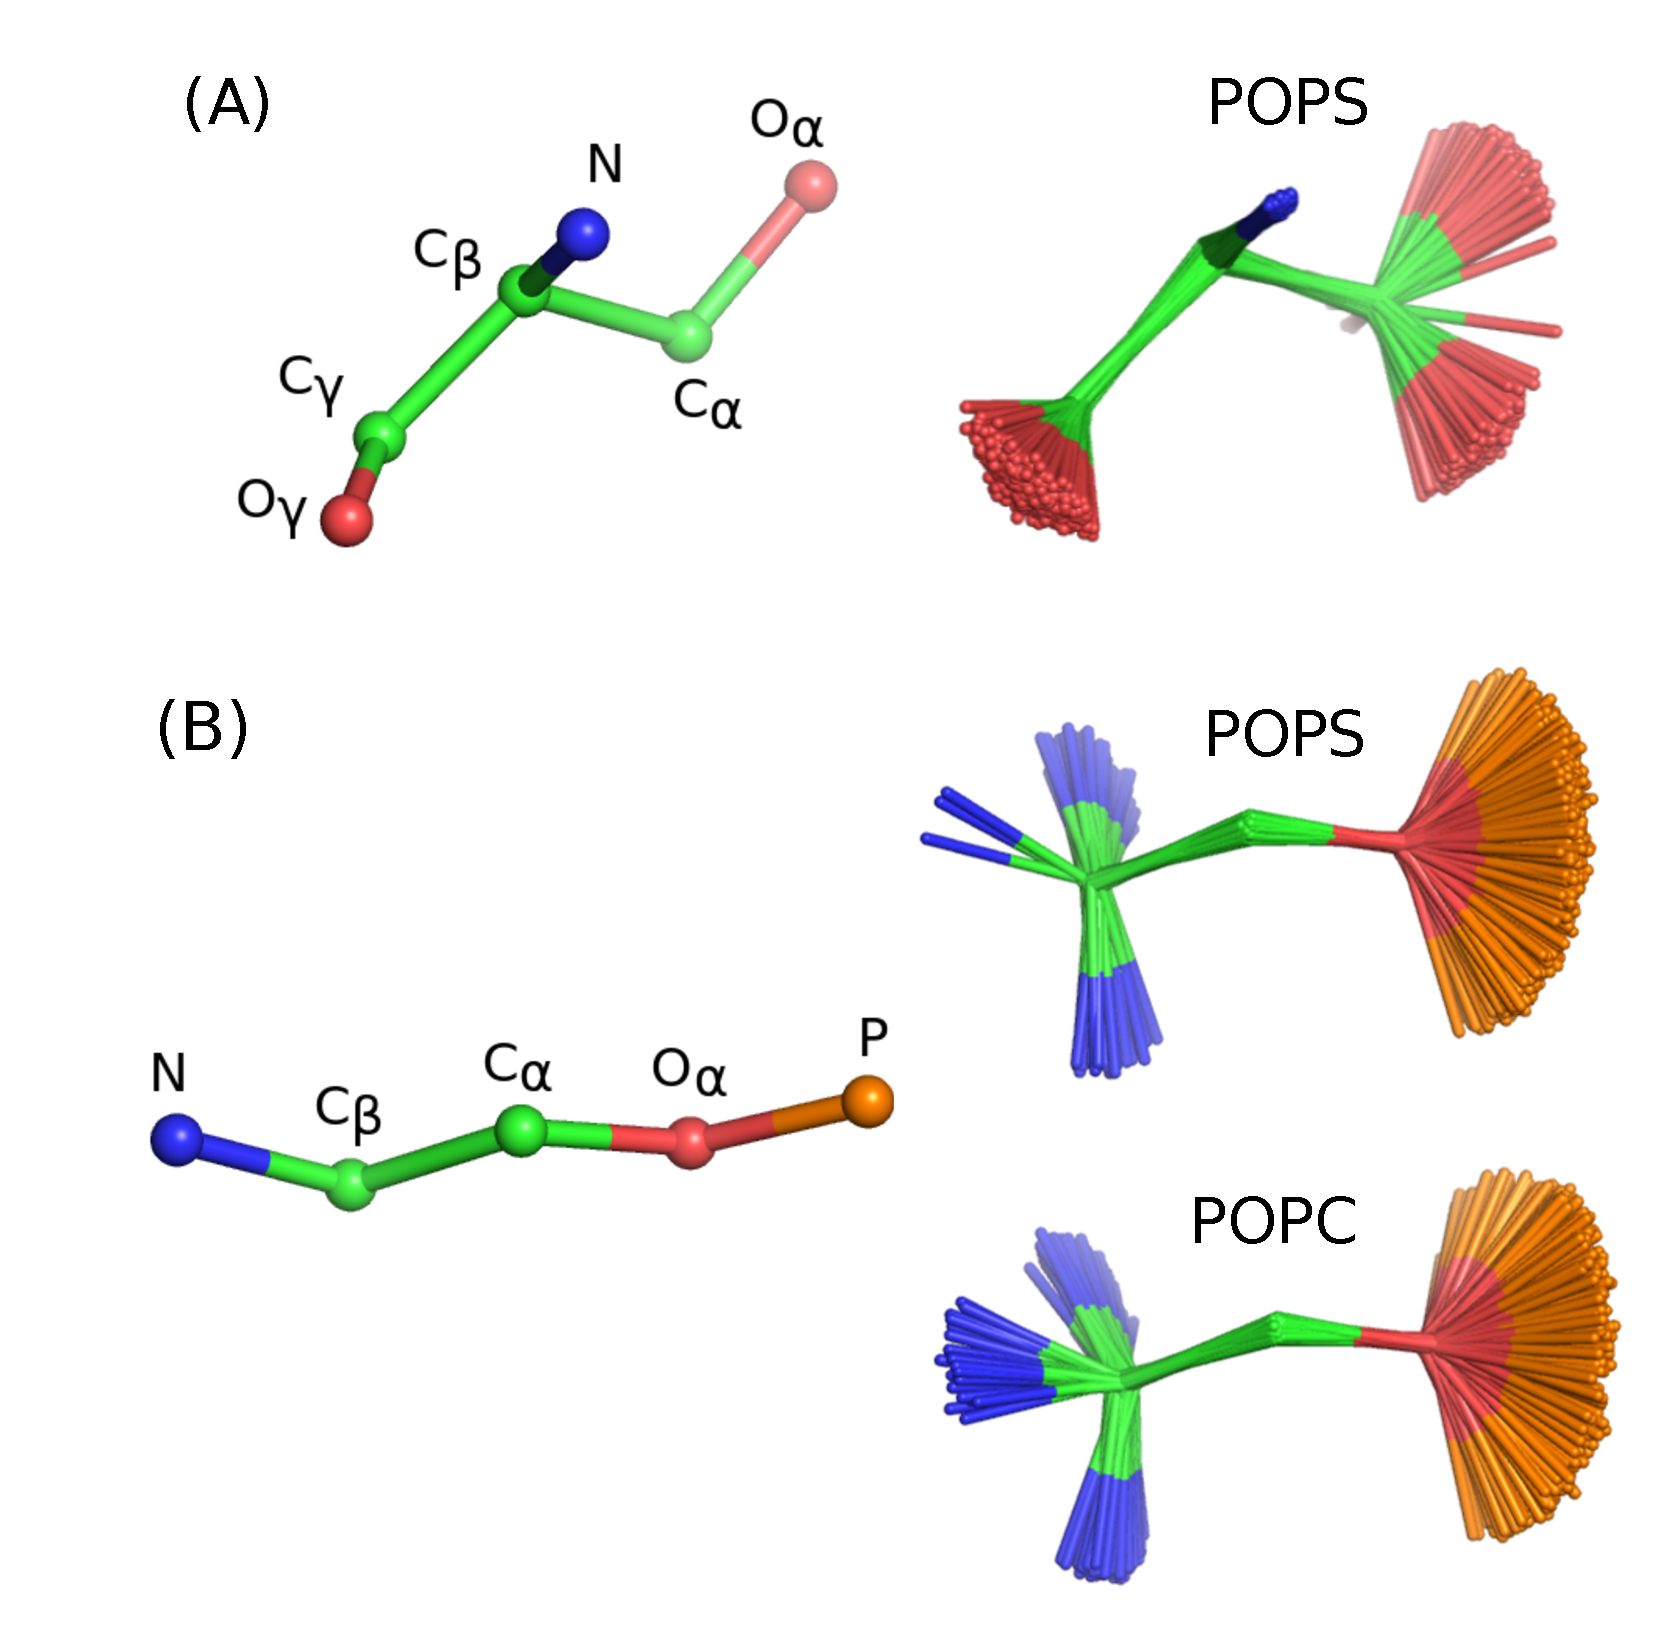
\includegraphics[width=9.0cm]{../Figs/structures.eps}
  \caption{\label{HGstructuresPSandPC}
    Overlayed snapshots from simulations conducted with CHARMM36 --- the force field producing the best agreement with experiments ---
     demonstrate the conformational fluctuations around
    (A) C$_\alpha$-C$_\beta$-C$_\gamma$-O$_\gamma$ and  O$_\alpha$-C$_\alpha$-C$_\beta$-N
    of PS headgroup and (B) N-C$_\beta$-C$_\alpha$-O$_\alpha$ and C$_\beta$-C$_\alpha$-O$_\alpha$-P
    dihedrals of PS and PC headgroups.
    The CHARMM36 POPC simulation is from Ref. \citenum{POPCcharmm36T303K} and Slipids POPC from Ref. \citenum{POPCslipids298K}.
  }
\end{figure}

\begin{figure}[]
  \centering
  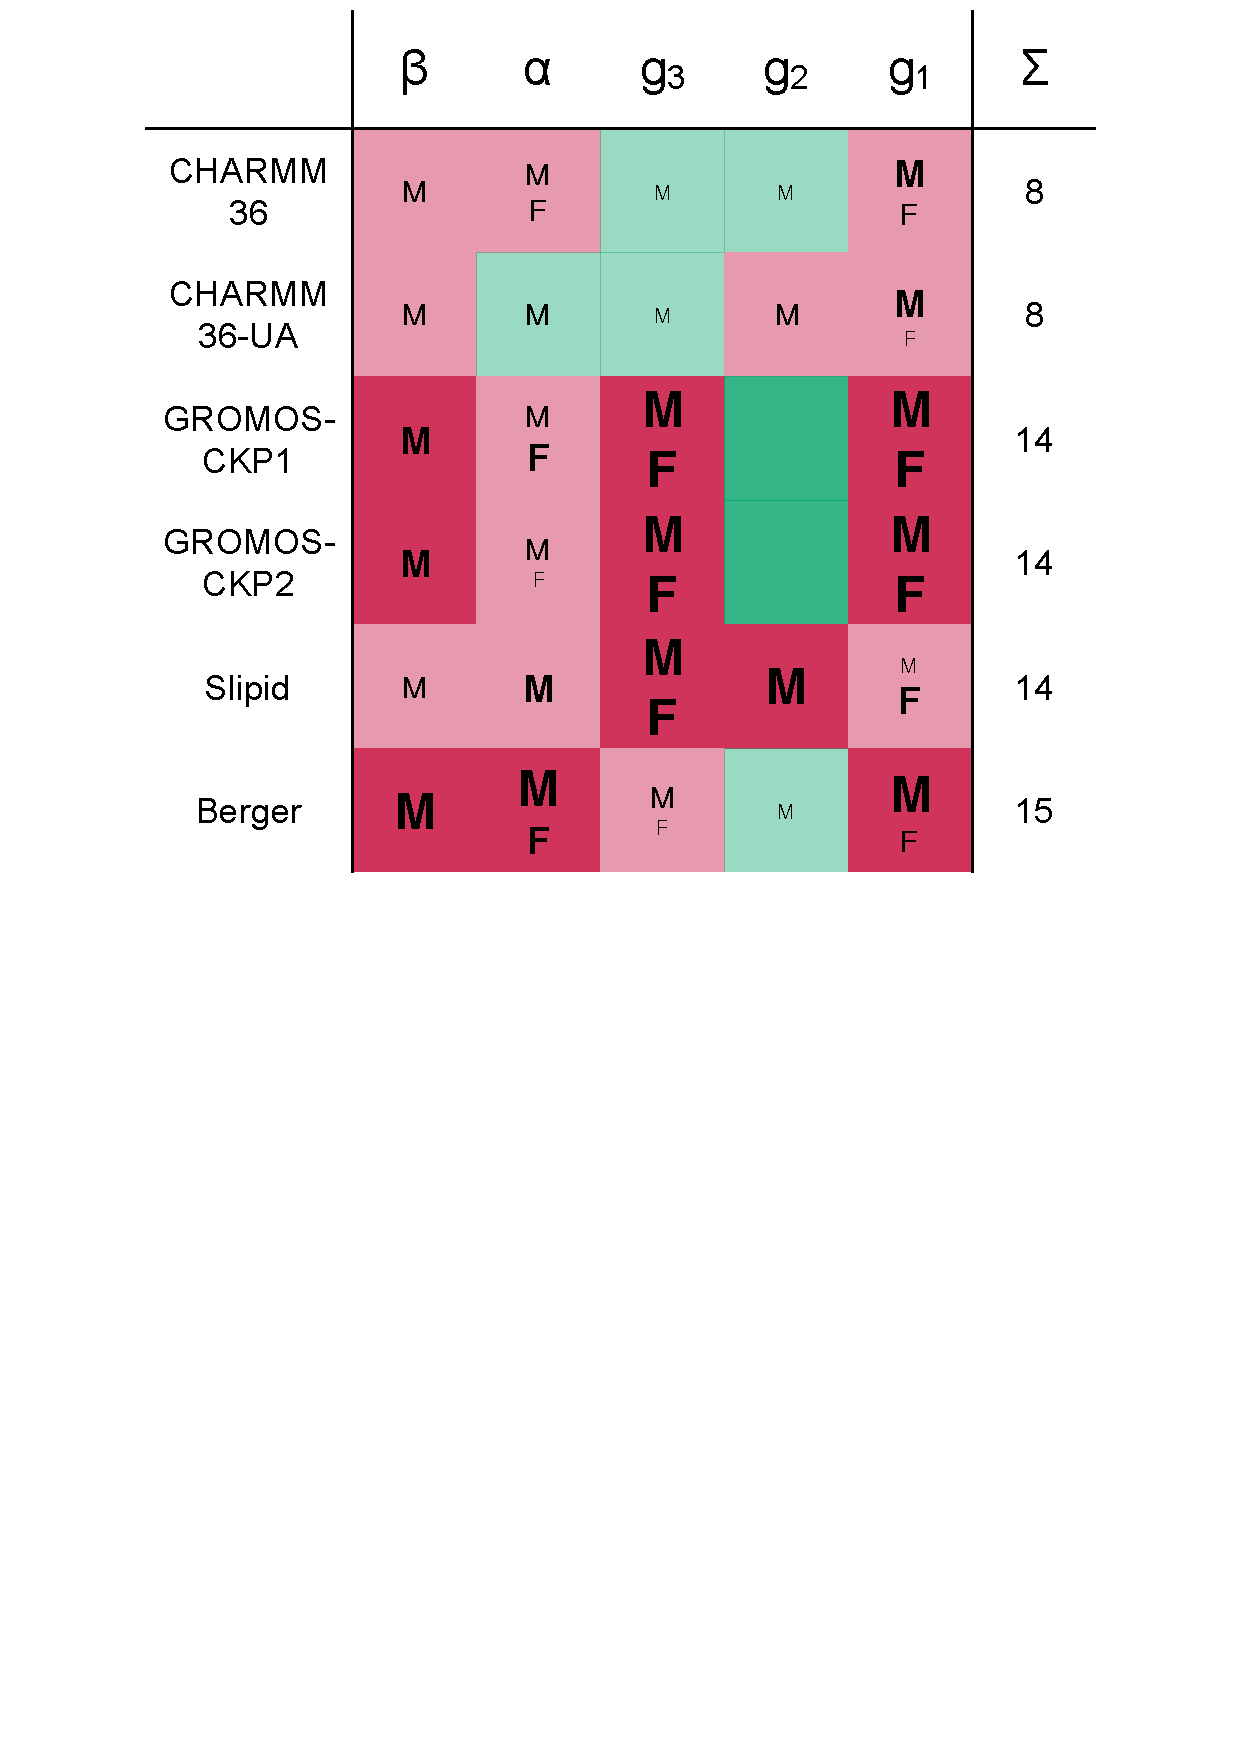
\includegraphics[width=9.0cm]{../Figs/comparisonTablePS.pdf}
  \caption{\label{comparisonTablePS}
    Rough subjective ranking of force fields based on Figure~\ref{HGorderParametersPS}.
    Here ÒMÓ indicates a magnitude problem, ÒFÓ a forking problem; letter size increases with problem severity. Color scheme: Òwithin experimental errorÓ (dark green), Òalmost within experimental errorÓ (light green), Òclear deviation from experimentsÓ (light red), and Òmajor deviation from experimentsÓ (dark red). The $\Sigma$-column shows the total deviation of the force field, when individual carbons are given weights of 0 (matches experiment), 1, 2, and 4 (major deviation). For full details of the assessment, see Supplementary Information.
  }
\end{figure}

The different PS MD models produce a wide variety of headgroup and glycerol backbone order parameters (Fig.~\ref{HGorderParametersPS})
and structures (Fig.~\ref{HGandGLYstructuresPS}) between different simulation models,
as previously observed also for PC lipids \cite{botan15}. None of the models produces a set of order parameters in full agreement with the experiments. The models perform generally less well for PS than for PC
(Figs.~\ref{HGorderParametersPS} and \ref{comparisonTablePS} vs. Figs. 2 and 4 in Ref.~\cite{botan15}).
which complicates the interpretation of structural differences between PC and PS headgroups.

\begin{figure}[!htb]
  \centering
  \includegraphics[width=9.0cm]{../Figs/NAdensPOPS.eps}
  \caption{\label{NAdensPOPS}
    Counterion densities of POPS lipid bilayer along the membrane normal from
    simulations with different force fields.
  }
  \todo{Commented by M. Javanainen in blog:
    MacRog pure POPS is simulated with Verlet cutoff scheme, Piggot is rerunning with group cutoff scheme. Check if affects results \& update figures when ready}
\end{figure}



However, concentrating on the headgroup, we see that the best performing models (Slipids, CHARMM36 and CHARMM36ua) do replicate the larger-than-in-PC forking of the $\alpha$-carbon \todo{observed in the experiments?} and the Slipids force field additionally correctly produces the significantly smaller $\beta$-carbon order parameter for PS compared to PC (Fig. \ref{HGorderParametersPS} vs. Fig. 2 in Ref.~\citenum{botan15}) \todo{refer to experiments also?}.

Interestingly, the C$_\alpha$-C$_\beta$-C$_\gamma$-O$_\gamma$  dihedral with
a single and narrow peak in the angle distribution close to 120$^{\circ}$ is more restricted
in the best three force field while other models give two maxima with different angles (Fig. \ref{dihedralsHG}).
The restricted motion is also visible in the sampled conformations (Figs.~\ref{HGstructuresPSandPC} (A) and \ref{HGandGLYstructuresPS})
suggesting that the rotation of the carboxyl group is limited in the serine headgroup.
In addition, the N-C$_\beta$-C$_\alpha$-O$_\alpha$ dihedral exhibits a more asymmetric
and restricted\todo{rather: narrow?} angle distribution for PS than for PC headgroup in
CHARMM36 simulations that have the best agreement with experiments
(Figs.~\ref{HGstructuresPSandPC} (B) and \ref{dihedralsHGpc}).
The results might reflect the increased rigidity anticipated\todo{detected, predicted, speculated?} in the early experimental studies \cite{browning80,buldt81}. %Also, the sampled conformations of glycerol backbone significantly vary between different simulation models (Figs. \ref{dihedralsGLY}, \ref{HGandGLYstructuresPS}, \ref{dihedralsGLYpc} and \ref{HGandGLYstructuresPSPC}),but further analysis is beyond the scope of this work which focuses on the PS headgroup. There is very little actual information in this statement. The variance was already noted above

The suggested characteristic conformations of the PS headgroup can be useful when interpreting experiments. However, as the none of the tested models fully reproduces the experimental order parameters, more accurate MD force fields are required to confirm the correct conformational ensemble.



\subsection{Counterion binding and interactions between PC and PS headgroups}\label{ciBINDINGsection}


\begin{figure}[!tb]
  \centering
  \includegraphics[width=8.0cm]{../Figs/HGorderparametersPCvsPS.eps}
  \caption{\label{HGorderparametersPCvsPS}
    Changes of POPC headgroup order parameters with increasing amount of POPS in POPC:POPS mixtures at 298~K.
    Experimental values are from Ref. \citenum{scherer87} with the signs measured in Ref.~\citenum{ferreira16}.
  }
  \todo{After we know which force field is used for POPC in Gromos-CKP simulations, we might be able to
    add Gromos-CKP data into this plot.}
\end{figure}

\begin{figure}[!tb]
  \centering
  \includegraphics[width=8.0cm]{../Figs/HGorderparametersPSvsPC.eps}
  \caption{\label{HGorderparametersPSvsPC}
    Changes of POPS headgroup order parameters with increasing amount of POPC in POPC:POPS mixtures at 298~K.
    Experimental values with the signs are measured for pure POPS system in this work.
    The signs are assumed to be the same for the mixture and the values are from Ref. \citenum{roux90}.
%    Since the experimental data of POPS in pure and diluted mixture come from
%    different experimental sets ($^{13}$C NMR in this work and $^{2}$H NMR in Ref. \citenum{roux90}),
%    the experimental change of the order parameter is less accurate than in typical measurements
%    where same technique is used in all conditions, see discussion about qualitative and quantitative 
%    accuracy in Ref. \citenum{ollila16}.
    The y-axis for the $\alpha$-carbon results of POPS (bottom) is transferred
    with the same value for both order parameters such that the lower order
    parameter value from pure POPS is at zero to correctly illustrate the significant forking.
  }
\end{figure}


Membranes containing PS lipids are always accompanied with counterions that
modulate electrostatic interactions between lipids and other biomolecules. 
Counterions are also suggested to screen the repulsion between charged lipid headgroups 
in MD simulations and thus to reduce the area per lipid of PS bilayers to be smaller than in PC
bilayers~\cite{pandit02,mukhopadhyay04,pedersen06}. 
Counterion density profiles along membrane normal 
indicate significant differences between force fields in both binding affinity
and distribution of ions in the interface (Fig. \ref{NAdensPOPS}).
The experimental area per lipid (62.7~\AA$^2$) \cite{pan14} 
is reproduced only in Gromos-CKP and in the MacRog simulation
with potassium counterions, while other models give significantly lower areas (Fig. \ref{NAdensPOPS}).
The counterion binding and the concomitant electrostatic screening of the headgroup
repulsion does not fully explain the low area per molecule values,
because the MacRog simulation, which has the strongest sodium binding
(the lowest concentrations in bulk water), gives the same area per molecule
as the CHARMM36ua simulation, which has significantly weaker counterion binding
affinity. On the other hand, changing counterions from sodium to potassium, having weaker binding
affinity, increases the area per molecule from 53~\AA$^2$ to 63~\AA$^2$ in MacRog simulations.
In conclusion, the results are in line with the previous study suggesting that the
low areas per molecule in PS lipid bilayers originate from the combination
of both counterion binding and hydrogen bonding network between lipid
headgroups \cite{petrache04}.

\begin{figure*}[ht]
  \centering
  \includegraphics[width=18cm]{../Figs/CHANGESwithCaClPS.eps}
  \caption{\label{changesWITHCaClPS}
    Changes of POPC (left) and POPS (right) headgroup order parameters from POPC:POPS (5:1) mixture
    as a function CaCl$_2$ concentration from experiments \cite{roux90} and different simulations
    at 298K (except the data for Berger model is from simulation of POPC:POPS (4:1) mixture at 310K \cite{ollila07a,melcrova16}). 
    The order parameter values from systems without calcium are set as the zero point of y-axis,
    except for the $\alpha$-carbon order parameter of POPS (bottom, right) for which the both order parameters are shifted
    such that the lower order parameter is zero without additional ions to correctly illustrate
    the forking with different concentrations of calcium.
    Potassium counterions are used in MacRog simulations and sodium counterions in Lipid14/17 simulations.
    In CHARMM36 and Berger simulation with added calcium, the charge is neutralized with calcium and monovalent counterions are not present.
  }
%  \todo{Upcoming simulations with original CHARMM36 have been mentioned in the blog:
%    http://nmrlipids.blogspot.com/2017/12/nmrlipids-iv-current-status-and.html?showComment=1520090718976\#c5569269391707740056.
%  these are not necessary, but could be added here if delivered.} \\
\end{figure*}



Binding of cations to zwitterionic PC lipid bilayers has been previously
evaluated against experiments using the changes of headgroup order parameters
as a function of salt concentration \cite{catte16}.
Studying binding of cations to negatively charged lipid bilayers is less straighforward,
because the cationic counterions are always present and the ion-free reference state does thus not exist.
In addition, the analysis is complicated by the artificial aggregation of counterions
in solution observed in some simulations (section \ref{mixtureTOadditionalCIs} in the supplementary information).
Therefore, we evaluate here the amount of bound charge not by adding salt
(although also this is discussed in the section \ref{mixtureTOadditionalCIs} in the supplementary information),
but by studying the changes of the headgroup order parameters with increasing amount of
negatively charged lipids (and thus increasing amount of cationic counterions) in the bilayer.
According to the molecular electrometer concept, the headgroup order parameters of POPC
increase when negatively charged POPS lipids are incorporated in lipid bilayer
(section \ref{HGorderparametersPCvsPEPSPGchol})~\cite{seelig87,scherer87}.
This is reproduced in the MacRog simulations with potassium counterions (Fig. \ref{HGorderparametersPCvsPS}),
which have the weakest binding affinity to POPS lipid bilayers (Fig.~\ref{NAdensPOPS}).
The CHARMM36 and Berger simulations predict no change, or a decrease,
in the POPC headgroup order parameters as a function of increased amount of POPS (Fig. \ref{HGorderparametersPCvsPS}).
This can be explained by the stronger counterion binding affinity, which cancels
the effect of negatively charged headgroups and prevents the experimentally observed
increase of headgroup order parameters with increasing amount of PS lipids.
Therefore, we suggest that the relatively weak binding of potassium
in the MacRog simulations (Fig. \ref{NAdensPOPS}) predicts the most
realistic surface charge density in membranes containing PS lipids,
while the other tested simulation models overestimate the counterion
binding affinity. The results are in line with the changes of headgroup order
parameters as a function of added counterions analyzed in section \ref{mixtureTOadditionalCIs}
in the supplementary information.

The reduced forking of the POPS $\alpha$-carbon (Fig.~\ref{HGorderparametersPSvsPC})
together with other experimental results suggest less rigid structure of PS headgroups when diluted with
POPC~\cite{browning80,buldt81,roux90,roux91,scherer87}.
None of the tested models reproduce the changes of POPS headgroup order
parameters with increasing amount of POPC in POPC:POPS mixtures (Fig. \ref{HGorderparametersPSvsPC}).
Therefore, we conclude that more accurate force fields are necessary
to correctly describe the PC-PS headgroup interactions in MD simulations.


\subsection{Ca$^{2+}$ binding affinity to bilayers with negatively charged PS lipids}
\begin{figure}[tb]
  \centering
  \includegraphics[width=9cm]{../Figs/CAdensPCPSmixtureLOWcons.eps}
  \caption{\label{CAdensPCPSmixture}
    Number density profiles of Ca$^{2+}$ from POPC:POPS (5:1) mixtures simulated with different force fields.
    The smallest simulated CaCl$_2$ concentrations are shown.
    For the density profiles from all the simulated concentrations see figure \ref{CAdensPCPSmixtureALL}
    in the supplementary information.
  }
  \todo{Should we include also counterions into the plot?} \\
\end{figure}

Calcium binding affinity to membranes containing the negative charged PS lipids can be
experimentally measured by detecting the PC lipid headgroup order parameters
from POPC:POPS (5:1) mixtures (section~\ref{electrometerFORmixtures}),
where the dehydrated lipid-ion complexes and phase separation are 
not observed~\cite{feigenson86,mattai89,roux90,roux91}.
Despite the lack of an ion-free reference state
in the presence of negatively charged lipids, our simulations give
coherent results for POPC headgroup order parameters as a function of
CaCl$_2$ in the POPC:POPS (5:1) mixtures (Fig. \ref{changesWITHCaClPS}).
As expected from the previous study of pure PC lipid
bilayers \cite{catte16}, almost all the tested simulation models overestimate the
experimentally observed~\cite{roux90} decrease of the POPC headgroup order parameters
in POPC:POPS (5:1) mixtures as a function of Ca$^{2+}$ concentration (Fig. \ref{changesWITHCaClPS}),
indicating overestimated calcium binding affinity.
The only exception is the CHARMM36 model with the NBfix
interaction employed for calcium~\cite{kim16}, which underestimates the changes in order parameters, 
indicating weaker binding affinity than experiments.
%incorporated in the parameters give by the CHARMM-GUI at the time of running the simulations (January 2018),
Notably, CHARMM36 simulations with the NBfix corrections \cite{venable13,kim16} give similar binding affinities of
calcium and sodium to POPC bilayer (see section \ref{CHARMMcalciumNBfix}), in contrast to the experimental 
data~\cite{cevc90,akutsu81,altenbach84}. Therefore, we conclude that the calcium binding affinity
is underestimated in CHARMM36 simulations with the NBfix for calcium \cite{kim16}, but overestimated 
in all the other tested models. This is evident in the calcium density distributions
along membrane normal, where almost all Ca$^{2+}$ ions bind to the membrane interface in
all simulation models except CHARMM36 (Fig. \ref{CAdensPCPSmixture}).


The headgroup order parameters of POPS experimentally measured from a POPC:POPS (5:1) mixture
exhibit a strong dependence of CaCl$_2$ with small concentrations and rapid saturation
below 100 mM (Fig. \ref{changesWITHCaClPS}).
In experiments, the order parameter of the POPS $\beta$-carbon increases with added CaCl$_2$,
whereas the larger $\alpha$-carbon order parameter decreases; a slight increase is observed in
the smaller $\alpha$-carbon. All these changes are significantly overestimated in the
tested simulation models, including CHARMM36 with underestimated binding affinity.
In addition, different simulation models predict qualitatively different behaviour
for the POPS $\alpha$-carbon order parameters with added calcium.
For example, both order parameters decrease in Berger, but increase
in MacRog, and in Lipid14/17 and CHARMM36 a more complicated behavior is seen.
This is in contrast to the PC headgroup, where
qualitatively correct reponse to bound ions is observed
in all simulation models, despite significant discrepancies in the headgroup
structure without additional ions~\cite{catte16}. Therefore, we conclude that
improvement of force fields is necessary to correctly describe interactions between the
PS headgroup and calcium ions in MD simulations.

\section{Conclusions}
Lipids with PS headgroups, and their interactions with ions,
play an important role in lipid-mediated signaling
processes \cite{leventis10,yeung08}. Recent studies using MD
simulations to interpret the various spectroscopic data
give contradictory results for the calcium binding details to PS
headgroups \cite{melcrova16,valentine18,hallock18}.  
Here, as was previously done for PC lipids \cite{botan15,catte16},
we used the headgroup C--H bond order parameters and the open collaboration approach to evaluate the quality
of the headgroup structure and ion binding affinity to PS lipids
in available MD force fields.
The main advantage of this approach is the direct connection
between the accurately measured experimental order parameters and the simulations,
which reduces the ambiguity in the interpretation of experiments.

First, we complemented the available experimental data of PS
lipid headgroup order parameters \cite{browning80,roux90} by measuring the signs of the order parameters.
Comparison to these data revealed that none of the available force fields
%tested using the NMRlipids open collaboration
was accurate enough to reproduce the PS
headgroup order parameters within the experimental accuracy. However,
the best models for the serine headgroup suggested a characteristic rigid conformation for its
carboxyl group. Comparison to the previously
measured headgroup order parameters from POPC:POPS (5:1) bilayers with different ion
concentrations \cite{roux90} then showed that the tested MD force fields
overestimate the cation binding affinity to the negatively charged bilayers
containing PS lipids with two exceptions. 1) The apparently most realistic monovalent ion binding
affinity to PS-containing lipid bilayers was observed in the MacRog
simulations with potassium counterions. 2) The CHARMM36 force field with the recently introduced
NBfix correction for calcium \cite{kim16} underestimated the calcium binding affinity.
The experimentally measured trends of the PS headgroup order parameter response
to the bound calcium, and to the dilution of bilayer with zwitterionic PC lipids, were not
qualitatively reproduced in any of the tested force fields, which indicates that improvements in
the MD force fields are necessary to study interactions between PS lipids and other biomolecules.
This is different to the previous results with PC lipids,
where the experimentally measured headgroup order parameter responses to the bound charge
were qualitative reproduced even though the headgroup structures themselves were
incorrect and the cation binding affinities overestimated \cite{catte16}.

Our results pave the way for the development of better MD force fields
for PS lipids. Using the headgroup order parameters, we were able to evaluate the
quality of various conformational ensembles in different force fields.
This can guide the development of force fields that would correctly reproduce the
conformations sampled by PS headgroups. The experimental dataset of headgroup order
parameters from POPC:POPS (5:1) mixture with different cation concentrations can
be used to improve cation binding details in the force fields, as recently demonstrated
for POPC using the electronic continuum correction \cite{melcr18}.
Similar study for POPS is being progressed separately \cite{ECCpops}.

% Tables may be be put in the text as floats.
% Here is an example of the general form of a table:
% Fill in the caption in the braces of the \caption{} command. Put the label
% that you will use with \ref{} command in the braces of the \label{} command.
% Insert the column specifiers (l, r, c, d, etc.) in the empty braces of the
% \begin{tabular}{} command.
%
% \begin{table}
% \caption{\label{} }
% \begin{tabular}{}
% \end{tabular}
% \end{table}

% If you have acknowledgments, this puts in the proper section head.
\begin{acknowledgments}
% Put your acknowledgments here.
  OHSO acknowledges financial support from Academy of Finland (315596),
  Integrated Structural Biology Research Infrastructure of
  Helsinki Institute of Life Science (Instruct-HiLIFE), and
  CSC-IT center for science for computational resources.
  MJ acknowledges financial support from the Emil Aaltonen foundation and
  and CSC-IT center for science for computational resources.
\end{acknowledgments}

\newpage


% Create the reference section using BibTe
\bibliography{refs.bib}

%\newpage
%\section{APPENDIX: The NMR results reported by Tiago Ferreira}

\listoftodos

\end{document}
%
% ****** End of file aiptemplate.tex ******
